Para a obtenção de um modelo inteligente capaz de verificar a autenticidade de assinaturas de indivíduos, é necessário, primeiramente, treiná-lo. Para tanto, é necessário um conjunto de exemplos, isto é, uma base de dados  que possua exemplos de assinaturas e seus respectivos rótulos, isto é, quando são forjadas ou genuínas, com vistas a prover características relevantes para o aprendizado.

Para este fim, utilizou-se dois conjuntos de dados originalmente disponibilizados pela
\emph{Signature Verification Competition} (SigComp 2009) realizada na \emph{International Conference on Document Analysis and Recognition} em 2009. Na ocasião da competição, cada um destes conjuntos de dados foi utilizado em uma etapa. Na etapa de treinamento, foi utilizado o conjunto de assinaturas do \emph{Norwegian Information Security laboratory and Donders Centre for Cognition} (NISDCC), composto originalmente de 1.920 assinaturas genuínas e forjadas. Para a etapa seguinte, de validação dos modelos submetidos, foi utilizado o conjunto coletado pelo \emph{Netherlands Forensic Institute} (NFI), composto por 1.953 novas assinaturas genuínas e forjadas \cite{icdar2009}. Considerando que a competição ocorreu há uma década, as bases de dados utilizadas na época são atualmente mantidas pela \emph{International Association for Pattern Recognition} (IAPR) e contam com um número de 1.898 assinaturas do conjunto NISDCC e 1.564 assinaturas do conjunto NFI \cite{iapr-tc11}. Esta versão mais recente é amplamente disponibilizada e, por essa razão, está sendo utilizada no escopo deste trabalho.

Os conjuntos disponibilizados pelo IAPR são compostos por dois tipos de assinaturas, as assinaturas \emph{offline} e as assinaturas \emph{online}. Nas assinaturas \emph{offline}, é considerado apenas o aspecto estático da mesma, ou seja, uma imagem obtida após o processo da assinatura ter sido concluído. Estes dados foram segmentados, inspecionados visualmente e, em seguida, pré-processados para fornecer imagens formatadas em cores, em escala de cinza e binárias com a resolução de $600$ dpi. Os dados das assinaturas \emph{online}, por sua vez, continham informações dinâmicas, que consistiam em arquivos de texto que descreviam os detalhes capturados em vários pontos durante o processo da assinatura, sendo estes as coordenadas $x$ e $y$ da ponta da caneta, a pressão exercida sobre a caneta, o ângulo azimutal e o ângulo de elevação \cite{icdar2009}. Um exemplo de uma assinatura \emph{offline} e a sua respectiva representação \emph{online} com os pontos plotados pode ser encontrada na Figura \ref{fig:sample-signature}.


\begin{figure}[h!]
\centering
\caption{Uma amostra das assinaturas \emph{offline} e \emph{online} do SigComp2009. Fonte: \cite{icdar2009}.}
\label{fig:sample-signature}
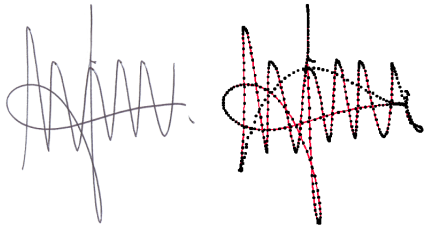
\includegraphics[width=0.5\textwidth]{imgs/sample-signature}
\end{figure}

Nestas bases de dados um certo autor produz várias versões de sua própria assinatura, compondo os exemplos de assinaturas genuínas. Várias pessoas foram convocadas a falsificar esta assinatura, produzindo os exemplos forjados das mesmas. Nestas falsificações utilizou-se a técnica \emph{over-the-shoulder}, na qual o autor forjador tem a oportunidade de visualizar a assinatura genuína antes da falsificação, podendo, inclusive, ter praticado anteriormente diversas vezes. Segundo Blankers et al., este tipo de falsificação costuma ser de difícil detecção \cite{icdar2009}.

Considerando a demanda por equipamentos específicos para obtenção das assinaturas \emph{online} e da pouca existência dos mesmos em cenários práticos, optou-se apenas pela utilização das assinaturas \emph{offline} para a elaboração deste trabalho, com vistas a concentrar os esforços em uma solução que incorpore aspectos de Visão Computacional. Após a exclusão destes exemplos, o quantitativo remanescente de assinaturas e seus tipos (genuína ou forjada) encontram-se disponíveis na Tabela \ref{tab:demonstracao-dataset}.

\begin{table}[h!]
	\centering
	\caption{Quantitativo de indivíduos e assinaturas \emph{offline} por conjunto de dados.}
	\label{tab:demonstracao-dataset}
\resizebox{\textwidth}{!}{
	\begin{tabular}{c C{2cm} C{2cm} C{3.25cm} C{2.5cm} C{2.5cm} C{2.25cm}}
		\toprule
		 \textbf{Conjunto}& \textbf{Autores originais} & \textbf{Autores forjadores} & \textbf{Autores originais com assinaturas forjadas} & \textbf{Assinaturas genuínas}  & \textbf{Assinaturas forjadas} & \textbf{Total de assinaturas} \\
		\midrule
		NISDCC & 12 & 31 & 12 & 60 & 1.838 & 1.898 \\
    NFI & 79 & 33 & 19 & 940 & 624 & 1.564 \\
		\bottomrule
	\end{tabular}}
\end{table}

Conforme pode ser observado, um mesmo autor produziu diferentes versões de sua assinatura. A coluna ``Autores originais'' indica o quantitativo destes indivíduos e a coluna ``Assinaturas genuínas'' indica o total de assinaturas feitas pelos mesmos. No caso do \emph{dataset} NISDCC, em especial, cada autor reproduziu sua própria assinatura $5$ vezes. No NFI não houve uma consistência quantitativa, mas, em média, foram $11$ reproduções da assinatura original pelo autor verdadeiro.

Ainda conforme a Tabela \ref{tab:demonstracao-dataset}, o NISDCC conta com $31$ autores forjadores, os quais produziram versões forjadas de todas as assinaturas originais, mas com um quantitativo de falsificações distintos para cada original, totalizando $1.838$ assinaturas forjadas com a técnica \emph{over-the-shoulder}. No caso do NFI, isto não ocorreu de mesma forma, pois apenas um subconjunto das originais foi alvo de falsificação.

Considerando o total exposto de assinaturas originais e forjadas, tendo sido compreendida a estrutura, organização e exemplos dos \emph{datasets}, partiu-se então para sua preparação com vistas a adequar seu uso para a solução proposta.
